\documentclass{article}
\usepackage{latexmldoc}
\newcommand{\LTXLaTeXML}{\pkg{LaTeXML}}
\newcommand{\LTXObject}{\pkg{LaTeXML::Object}}
\newcommand{\LTXToken}{\pkg{LaTeXML::Token}}
\newcommand{\LTXTokens}{\pkg[LaTeXML::Token]{LaTeXML::Tokens}}
\newcommand{\LTXNumber}{\pkg[LaTeXML::Token]{LaTeXML::Number}}
\newcommand{\LTXDimension}{\pkg[LaTeXML::Token]{LaTeXML::Dimension}}
\newcommand{\LTXMuDimension}{\pkg[LaTeXML::Token]{LaTeXML::MuDimension}}
\newcommand{\LTXGlue}{\pkg[LaTeXML::Token]{LaTeXML::Glue}}
\newcommand{\LTXMuGlue}{\pkg[LaTeXML::Token]{LaTeXML::MuGlue}}
\newcommand{\LTXBox}{\pkg{LaTeXML::Box}}
\newcommand{\LTXMathBox}{\pkg[LaTeXML::Box]{LaTeXML::MathBox}}
\newcommand{\LTXComment}{\pkg[LaTeXML::Box]{LaTeXML::Comment}}
\newcommand{\LTXList}{\pkg[LaTeXML::Box]{LaTeXML::List}}
\newcommand{\LTXMathList}{\pkg[LaTeXML::Box]{LaTeXML::MathList}}
\newcommand{\LTXWhatsit}{\pkg[LaTeXML::Box]{LaTeXML::Whatsit}}
\newcommand{\LTXFont}{\pkg{LaTeXML::Font}}
\newcommand{\LTXMathFont}{\pkg[LaTeXML::Font]{LaTeXML::MathFont}}
\newcommand{\LTXNode}{\pkg{LaTeXML::Node}}
\newcommand{\TextNode}{\pkg[LaTeXML::Node]{LaTeXML::TextNode}}
\newcommand{\LTXCommentNode}{\pkg[LaTeXML::Node]{LaTeXML::CommentNode}}
\newcommand{\LTXProcessingInstruction}{\pkg[Node]{LaTeXML::ProcessingInstruction}}
\newcommand{\LTXDocument}{\pkg[LaTeXML::Node]{LaTeXML::Document}}
\newcommand{\LTXDefinition}{\pkg{LaTeXML::Definition}}
\newcommand{\LTXExpandable}{\pkg[LaTeXML::Definition]{LaTeXML::Expandable}}
\newcommand{\LTXPrimitive}{\pkg[LaTeXML::Definition]{LaTeXML::Primitive}}
\newcommand{\LTXRegister}{\pkg[LaTeXML::Definition]{LaTeXML::Register}}
\newcommand{\LTXConstructor}{\pkg[LaTeXML::Definition]{LaTeXML::Constructor}}
\newcommand{\LTXParameters}{\pkg{LaTeXML::Parameters}}
\newcommand{\LTXParameter}{\pkg[LaTeXML::Parameter]{LaTeXML::Parameter}}
\newcommand{\LTXKeyVals}{\pkg[LaTeXML::Parameter]{LaTeXML::KeyVals}}
\newcommand{\LTXMouth}{\pkg{LaTeXML::Mouth}}
\newcommand{\LTXFileMouth}{\pkg[LaTeXML::Mouth]{LaTeXML::FileMouth}}
\newcommand{\LTXGullet}{\pkg{LaTeXML::Gullet}}
\newcommand{\LTXStomach}{\pkg{LaTeXML::Stomach}}
\newcommand{\LTXIntestine}{\pkg{LaTeXML::Intestine}}
\newcommand{\LTXModel}{\pkg{LaTeXML::Model}}

\title{\LaTeXML: a \LaTeX\ to \XML\ Converter; \emph{Preview}}
\author{Bruce R.~Miller}
\begin{document}
\maketitle
\section{Overview}
For many, \LaTeX\ is the prefered means for document authoring, particularly when
significant mathematical content is involved.
On the other hand, content-oriented \XML\ is an extremely useful storage format
allowing documents to be used, and reused, for a variety of purposes, not least, 
presentation on the Web.  Given the rough mismatch between the two,
particularly for mathematics, conversion  from \LaTeX\ to \XML\ is a bit tricky.
Faced with this situation, and the lack of other suitable tools at that time,
the \URL[Digital Library of Mathematical Functions]{http://dlmf.nist.gov}
proceeded to develop thier own tool, \LaTeXML, to fill this need.
This document describes a \emph{preview} release of \LaTeXML.

The idealistic goals of \LaTeXML\ are:
\begin{itemize}
\item Faithful emulation of \TeX's behaviour.
\item Easily extensible.
\item Lossless; preserving both semantic and presentation cues.
\item Uses abstract \LaTeX-like, extensible, document type.
\item Determine the semantics of mathematical content\\
    (Content \MathML, \emph{Good} Presentation \MathML, eventually \OpenMath).
\end{itemize}

As these goals are not entirely practical, or somewhat contradictory,
they are implicitly modified by ``as much as possible.''
Completely mimicing \TeX's behaviour would seem to require the sneakiest modifications
to \TeX, itself.  `Ease of use,' of course, is in the eye of the beholder.
Few documents are likely to have completely unambiguous mathematics markup; 
human understanding of both the topic and the surrounding text is needed to
properly interpret any particular mathematical fragment.
Thus, we expect that document-specific declarations or tuning to be necessary
to faithfully convert mathematical documents, rather than presuming to
provide a `turn-key' solution. At the same time, we would encourage
a more content-oriented mathematical markup style, than a presentation-oriented style.

\medskip
This document continues with an overview of the usage of \LaTeXML (\S\ref{sec:usage})
and its architecture (\S\ref{sec:architecture}).   
In \S\ref{sec:packages}, an overview of customizing \LaTeXML\ is given.
How mathematics is converted to content-oriented forms is discussed in \S\ref{sec:math}.
Finally, Appendix \ref{app:architecture} gives slightly more details about the architecture,
Appendix \ref{app:hierarchy} shows an object hierarchy of the system
and Appendix \ref{app:todo} lists the main problem areas and unfinished features.
In general, for more detail, you should see the perl documentation of various
\LaTeXML\ Packages, or the source code and examples, themselves.

\section{Using \LaTeXML}\label{sec:usage}
The basic conversion to \XML\ (using the \LaTeXML\ DTD, by default) is carried out
by the command:
\begin{quote}
 \cmd{latexml \textit{options} document.tex > document.xml}
\end{quote}
The more useful command options are
\begin{description}
\item[\cmd{--output}=\textit{outputfile}]
Specifies the output file; by default the XML is written to stdout.

\item[\cmd{--preload}=\textit{module}]
Requests the loading of an optional module or package.  This may be useful if the TeX code
does not specificly require the module (eg. through input or usepackage).

\item[\cmd{--path}=\textit{dir}]
Add \textit{dir} to the search paths used when searching for files, modules, style files, etc;
somewhat like TEXINPUTS.  This option can be repeated.

\item[\cmd{--quiet}]
Reduces the verbosity of output during processing, used twice is pretty silent.

\item[\cmd{--verbose}]
Increases the verbosity of output during processing, used twice is pretty chatty.
Can be useful for getting more details when errors occur.

\item[\cmd{--strict}]
Specifies a strict processing mode. By default, undefined control sequences and
invalid document constructs (that violate the DTD) give warning messages, but attempt
to continue processing.  Using \cmd{--strict} makes them generate fatal errors.

\item[\cmd{--VERSION}]
Shows the version number of the LaTeXML package..
\end{description}
See \cmd{latexml --help} for other options that may be useful for debugging.

Additional transformations, particularly the parsing of mathematical content, are carried out
by the postprocessor \cmd{latexmlpost}:
\begin{quote}
\cmd{latexmlpost \textit{options} document.xml}
\end{quote}
where the options are:
\begin{description}
\item[\cmd{--stylesheet=\textit{stylesheet}}] requests an \texttt{XSLT} transformation of
    the \XML\  using the given stylesheet.
\item[\cmd{--format=(html|xhtml)}]  Specifies the format for conversion. Default
    is to leave as \XML.
\item[\cmd{--destination=\textit{file}}]  Specifies the file to write the output.
    If the file has either an html or xhtml extension, that format is assumed.
\item[\cmd{--source=\textit{dir}}] Some postprocessing (eg. transforming graphics files)
     may need access to the directory  where the original \TeX\ file resided 
     (if it isn't the current working directory).
\item[\cmd{--verbose}] Increases the amount of messages about the progress of processing.
\item[\cmd{--help}] Prints a brief description of the command and options.
\end{description}
Transforming to html format involves parsing math formula and converting them to Presentation MathML,
transforming tables into an HTML consistent format, converting graphics files and applying 
an XSLT transformation.
Transforming to html format is similar, but math formula are converted to images.
If no format is specified, only math parsing and conversion is done.

\section{Architecture}\label{sec:architecture}
Like \TeX, \LaTeXML\ is data-driven: the text and control sequences\footnote{\TeX's name
for the backslashed commands; ie.~macros, primitives and so forth}
in the source file (and packages used, being simply collections of macros)
direct the processing.
You exert control over the processing, and customize it, by 
the \emph{implementation} of the control sequences (or packages).
That, or by postprocessing --- all the heavy-lifting that implements parsing 
of mathematics is carried out in postprocessing\footnote{But note that it is planned,
in the next version, to move the parsing, along with dealing with math declarations, 
back into \cmd{latexml}; Then \cmd{latexmlpost} will only deal with XSLT and transformations
of the format of math (eg. MathML)}; See \S\ref{sec:math}.


\begin{figure}[tb]
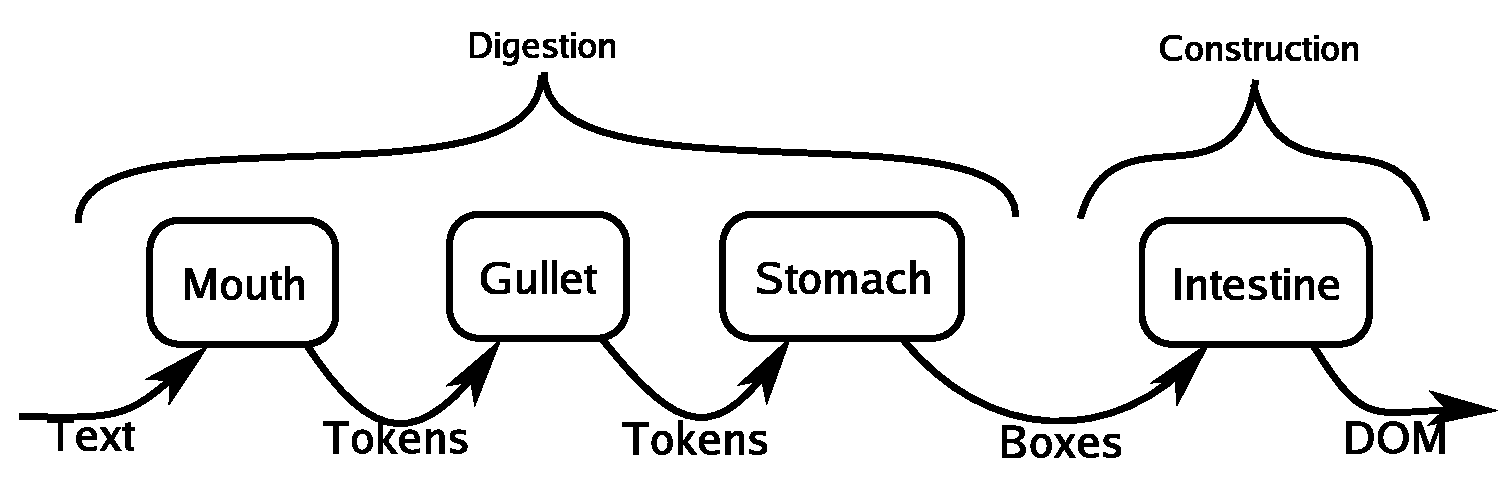
\includegraphics[width=\columnwidth]{dataflow}
\caption{Flow of data through \LaTeXML's digestive tract.\label{fig:dataflow}}
\end{figure}
The top-level class, \LTXLaTeXML, manages the processing.
Roughly, \TeX's digestive tract is emulated as follows; See Figure \ref{fig:dataflow}.
The processing is broken into two phases; digestion and construction.
The \emph{Stomach}  maintains the current state of processing during digestion;
The \LaTeXML\ object sets up a chain consisting of a stomach, a 
\emph{Mouth} (to convert characters from the file into \emph{Tokens}; see \ref{sec:tokenization}) 
and a \emph{Gullet} (to read tokens from that Mouth, expanding any macro or expandible
tokens in the process; see \ref{sec:expansion}).
The stomach then reads tokens from the gullet and digests them
(executing \emph{Primitives} and  converting the remaining tokens into \emph{Boxes},
\emph{Lists} and \emph{Whatsits}; see \ref{sec:digestion}).
These three components operate in \emph{pull mode}, each pulling data from the previous.

Document construction is carried out by the \emph{Intestine}, which recursively traverses 
the digested boxes constructing an intermediate tree representing the \XML\ document tree.
As a last step, the intermediate tree is converted to an \code{XML::LibXML} document,
which can be output or processed further.

The key features for generating \XML, are the control sequences that we
call \emph{Constructors} which encode the construction of arbitrary \XML\ fragments,
and our extension of the concept of a Whatsit to represent the digested form of constructors.

This process is described in slightly more detail in Appendix \ref{app:architecture}, but
see the perl documentation \cmd{perldoc} for the modules for the APIs, and, ultimately,
the source for full details.


\section{Packages: Implementing Control Sequences}\label{sec:packages}
The processsing of the \LaTeX\ document and its  conversion into \XML\ is affected
by the definitions of control sequences, either as macros, primitives or constructors, 
and other declarations specifying the document type, properties of \XML\ tags, ligatures, \ldots.
These definitions and declarations are typically contained in `packages' which provide
the implementation of \LaTeX\ classes and packages.  For example, the \LaTeX\ directive
\verb|\usepackage{foo}| would cause \LaTeXML\ to load the file \code{foo.ltxml}.
This file would be sought in any of the directories in perl's \verb|@INC| list (typically
including the current directory), or in a \verb|LaTeXML/Package| subdirectory of any of 
those directories.  If no such file is found, \LaTeXML\ would look for \code{foo.sty} and
attempt to process it.

When processing a typical file, say \textit{jobname}\texttt{.tex}, 
the following packages are loaded:
\begin{enumerate}
\item the core \code{TeX} package
\item any packages named with the \verb|--preload| option,
\item a file \textit{jobname}\texttt{.latexml}, if present;
      this provides for document-specific declarations.
\end{enumerate}
Document processing then commences; by default, \LaTeXML\ assumes that the document is plain \TeX.
However, if a \verb|\documentclass| directive is encountered, the \code{LaTeX} package, as well
as a package for the named document class are loaded.

\LaTeXML\ implementations are provided for a number of the standard \LaTeX\ packages,
although many implement only part of the functionality.  Contributed implementations are,
of course, welcome.  These files, as well as the document specific \textit{jobname}\texttt{.latexml},
are essentially Perl modules, but use the facilities described in \perldoc{LaTeXML::Package}.

\section{Mathematics}\label{sec:math}
The mathematical material is parsed into a content-oriented representation following
the usual steps: lexical scanning, grammar-based parsing and (eventually) type-analysis, but
with a few twists. As \LaTeXML\ constructs the initial document, the mathematical material
is converted mainly into a sequence of lexical (mathmematical) tokens (\tag{XMTok}), 
possibly carrying extra information such as name, grammatical role, font, style, etc.  
The exceptions are where the mathematical structure is clear from the markup itself, 
such as \verb|\frac| or sub- and superscripts, where a generalized \emph{application} (\tag{XMApp})
is constructed.  The substructures will typically play no role in the parsing of the upper 
layer of tokens; they are wrapped (in an \tag{XMArg} or \tag{XMWrap} element) and parsed
as separate subexpressions.  Thus we speak of \LaTeXML\ as being a \emph{structure preserving lexer}.  

The parser, invoked by the postprocessor, works only with the top-level lists of lexical tokens,
or with those sublists contained in an \tag{XMArg}.  The grammar works primarily through
the name and grammatical role.  The name is given by an attribute, or the content if it is
the same.  The role (things like ID, FUNCTION, OPERATOR, OPEN, \ldots) is also given
by an attribute, or, if not present, the name is looked up in a document-specific
dictionary (\textit{jobname}\texttt{.dict}), or in a default dictionary.

Additional exceptions that need fuller explanation are: 
(1) \LTXConstructor s may wish to create a dual object (\tag{XMDual}) whose children are 
the semantic and presentational forms.
(2) Spacing and similar markup generates \tag{XMHint} elements, which are currently ignored
during parsing, but probably shouldn't.

\appendix
\section{Architectural Details}\label{app:architecture}
\subsection{Tokenization}\label{sec:tokenization}

\paragraph{\LTXMouth}
Given a string or file, a mouth tokenizes the input text according to
the current category codes in the \LTXStomach. Category codes distinguish classes of characters
such as plain characters, control sequences,  active characters and \TeX's special characters  
for grouping,  sub- and super-script and math mode.  The main method is \method{readToken}, which
returns the next \LTXToken\ from the input.  A \LTXFileMouth\ is a mouth for reading from a file.


\paragraph{\LTXToken, \LTXTokens} These packages represent a Token (a pair containing a character
or string and the category code), and a list of tokens, respectively.  The latter responds to the same
interface as \LTXMouth, so it can also be read from.

\subsection{Expansion}\label{sec:expansion}

\paragraph{\LTXGullet}
The gullet reads tokens from the mouth, possibly expanding them.
The main methods are \method{readToken} and  \method{readXToken}.
The latter returns the next unexpandable token from the input;
if the token's current meaning in the \LTXStomach\ is an \LTXExpandable\ (a macro
or other expandable control sequences),
it is expanded and its expansion is replaced in the input before retrying.
The driving \LTXLaTeXML\ instance binds the exported variable \code{\$GULLET} to the current gullet.

\paragraph{\LTXExpandable} Instances (subclass of \LTXDefinition)
represent the expansions of control sequences. Expandables typically are used for
conditionals (like \verb|\if|, \verb|\ifx|, \ldots) and built-in control sequences that expand 
into sequences of tokens (such as \verb|\jobname|). The arguments are read from the gullet,
and used in generating the replacement tokens.

\subsection{Digestion}\label{sec:digestion}
\paragraph{\LTXStomach}  The Stomach maintains global state during digestion and carries 
out the digestion of tokens. The top-level method \method{readAndDigestFile(\$file)} 
sets up the initial state and stack, pre-loads packages (at least \code{TeX}), and then digests
all available input, returning the digested \LTXList.
The driving \LTXLaTeXML\ instance binds the exported variable \code{\$GULLET} to the current gullet.

The mouth and gullet refer to the stomach to set or access the mode, various values and
definitions. To mimic \TeX's binding of definitions and values scoped by grouping, 
the stomach maintains a stack of the active bindings for each control sequence, along with the
bindings to be undone on the next end-group; this allows the most common operations to be carried
out in linear time.

Basically, there are four cases when digesting a \LTXToken:
 \begin{itemize}
  \item A plain character is simply converted to a \LTXBox (or \LTXMathBox\ in math mode), 
   recording the current \LTXFont.
  \item If a control sequence represents \LTXPrimitive, the primitive is invoked, executing its
   stored subroutine.  This is typically done for side effect (changing the state in the stomach), 
   although they may also contribute digested material.
   As with macros, any arguments to the primitive are read from the gullet.
  \item Grouping (or environment bodies) are collected into a \LTXList\ (or \LTXMathList\ in math mode).
  \item A special class of control sequence, called a \LTXConstructor\ produces a 
   \LTXWhatsit\ which remembers the control sequence and arguments that
   created it, and defines its own translation into \XML\ elements, attributes and data.
   Arguments to a constructor are read from the gullet and also digested.
 \end{itemize}
Finally, \code{Filter}s are applied to the resulting lists (see below).

\paragraph{\LTXBox, \LTXMathBox, \LTXList, \LTXMathList, \LTXWhatsit} Instances of
these classes represent the digested objects: boxes being characters; lists being sequences
of digested objects; whatsits representing some sort of document fragment.
Note that, currently, Although \verb|\par| tends to do the `right thing', there 
is no real notion of horizontal or vertical mode.

\paragraph{\LTXPrimitive, \LTXConstructor} These subclasses of \LTXDefinition are carried out
(at least partly) in the stomach. They may have before and after daemons; little bits
of code that affect the state.  A primitive is carried out for only side-effect,
but a constructor generates a whatsit that survives to the \LTXIntestine.

\paragraph{\code{Filter}} Filters are roughly a generalization of ligatures. They are matched
against sequences of digested items during digestion; if they pattern is matched, it is substituted
by the replacement.  They are currently defined for the kinds of substitutions that would
make sense for \XML; namely repeated characters like \texttt{-} or \texttt{`} are replaced by 
the appropriate unicode. Also, in math, patterns of digits or letters (in non-mathitalic fonts) 
are combined as one would expect.  On the other hand, ligatures like \texttt{ffi} do not
really seem appropriate here --- or do they? --- they would be easily implemented, but
they might adversely affect search.

\subsection{Construction}\label{sec:construction}
\paragraph{\LTXIntestine}
The intestine traverses the recursive \LTXList\ of digested \LTXList s, 
\LTXBox es and \LTXWhatsit s, constructing a (\LTXDocument),
according to the current \LTXModel.  Generally, a \LTXBox\ gives rise to text data, whereas
a \LTXWhatsit\ describes a document fragment (consisting of elements, thier attributes and or content).
At each insertion, the \LTXModel\ is consulted to determine if the insertion is allowed at the
current point, or if intermediate elements may need to be opened or closed.
This allows the document structure of sections and paragraphs to be automatically
constructed, for example, even though \LaTeX\ doesn't explicitly close \verb|\section|,
nor open \verb|\par|.
(See \perldoc{LaTeXML::Intestine},  \perldoc{LaTeXML::Node},  \perldoc{LaTeXML::Model}).

\section{Object Hierarchy}\label{app:hierarchy}
\begin{description}
  \item[\LTXObject]: Abstract base class.
  \begin{description}
    % In Token.pm
    \item[\LTXToken]: A \TeX\ token: character/string with category code.
    \item[\LTXTokens]: A list of \LTXToken s.
    \item[\LTXNumber]: A \TeX\ number.
    \begin{description}
      \item[\LTXDimension]: A \TeX\ dimension; number with unit.
      \begin{description}
        \item[\LTXMuDimension]: A \TeX\ math-mode dimension.
        \item[\LTXGlue]:  A \TeX\ dimension with shrink and stretch.
        \begin{description}
          \item[\LTXMuGlue]: A \TeX\ math-mode glue.
        \end{description}
      \end{description}
    \end{description}
    % In Box.pm
    \item[\LTXBox]: A digested character/string; base class for digested objects.
    \begin{description}
      \item[\LTXMathBox]: A digested character token in math.
      \item[\LTXComment]: A digested comment.
      \item[\LTXList]: A list of text-mode boxes.
      \begin{description}
        \item[\LTXMathList]: A list of math-mode boxes.
      \end{description}
      \item[\LTXWhatsit]: A special digested object with arguments and properties; has its own
             rules for conversion into an document fragment.
    \end{description}
    % In Font.pm
    \item[\LTXFont]: A representation of a font, attached to digested objects.
    \begin{description}
      \item[\LTXMathFont]: A font in math; special rules for merging.
    \end{description}
    % In Node.pm
    \item[\LTXNode]:  Intermediate representation of an XML element (also base class).
    \begin{description}
      \item[\TextNode]: a text node. 
      \item[\LTXCommentNode]: a comment node.
      \item[\LTXProcessingInstruction]: a processing instruction
      \item[\LTXDocument]: the root document object.
    \end{description}
    % In Definition.pm
    \item[\LTXDefinition]: Represents the action of executable control sequences
    \begin{description}
      \item[\LTXExpandable]: A definition expandable in the Gullet, (eg.~a macro).
      \item[\LTXPrimitive]: Definition for primitives, carried out in Stomach.
      \begin{description}
        \item[\LTXRegister]: A definition for \TeX\ registers.
        \item[\LTXConstructor]: A definition that `constructs' document fragments;
             generates a Whatsit during digestion.
      \end{description}
    \end{description}
    % In Parameters.pm
    \item[\LTXParameters]: A definition's parameter list; a collection of \LTXParameter s.
    \item[\LTXParameter]: A definition's parameter, including type, optional, etc.
    \item[\LTXKeyVals]: Representation of \LaTeX-style Key-Value lists.
    % In Mouth.pm
    \item[\LTXMouth]: The organ that converts characters (eg.~from files) into \LTXToken s.
    \begin{description}
      \item[\LTXFileMouth]: A mouth that tokenizes input from a file.
    \end{description}
    % In Gullet.pm
    \item[\LTXGullet]: The organ that expands \LTXToken s into other sequences of tokens;
      also provides common `parsing' operations such as reading numbers, delimited lists of tokens, etc.
    % In Stomach.pm
    \item[\LTXStomach]: The organ that digests \LTXToken s, converting them to a tree of
       digested boxes; also contains the current state of grouping, bindings of definitions, etc.
    % In Intestine.pm
    \item[\LTXIntestine]: The organ that constructs the document tree from digested boxes.
       Vaguely analogous to \TeX's output routine, but runs at end of document, rather than per-page.
    % In Model.pm
    \item[\LTXModel]: Represents the model of the document, extracted from the DTD.
  \end{description}
\end{description}

\section{Issues and ToDo}\label{app:todo}
Lots\ldots!
\begin{itemize}
\item Lots of useful \LaTeX\ packages have not been implemented, and those
  that are aren't necessarily complete.
\item \TeX\ boxes aren't really complete, and in particular things like \verb|\ht0|
  don't work.
\item Possibly useful to override (pre-override?) a macro defined in the source file;
  that is, define it and silently ignore the definition given in the source.
\item \ldots um, \ldots \emph{documentation}!
\end{itemize}
\end{document}
